%%%%%%%%%%%%%%%%%%%%%%%%%%%%%%%%

% The post-genomic era

%%%%%%%%%%%%%%%%%%%%%%%%%%%%%%%%

\chapter[The post-genomic era]{\textbf{T}he post-genomic era}\label{sec:genomics}
\sectionblue*{Summary}
\begin{center}
\begin{tabular}{c}
\fcolorbox{blue}{verylightgrey}{
\begin{minipage}[][4cm][c]{0.8\linewidth}
\sffamily
%abstract 
This chapter is a basic survey of the molecular and cell biological concepts that will be used
throughout this thesis, with special emphasis on the topics of genetics and genomics. In addition, the 
relatively new discipline of bioinformatics is examined, focusing on the genomic databases 
and the integration of data from different biological domains. The dramatic changes that medicine 
and drug design are going to experience after the sequencing of the human genome project are explored 
at the end of the chapter.
\end{minipage}}\\
\\[2ex]
\begin{minipage}[][4cm][c]{0.9\linewidth}
\minitoc
\end{minipage}
\end{tabular}
\end{center}
\newpage


\sectionblue{The genomic landscape}\label{sec:glandscape}

\subsectionblue{The universe of the cells}
\index{cell}% 

\lettrine[lines=4,loversize=-0.1,lraise=0.1,lhang=.2]{T}{he cell}, a small membrane-bounded 
compartment filled with a concentrated aqueous solution of chemicals, is the essential constituent
of life. Bacteria, plants, birds or humans, all living organisms on Earth 
are made of at least one cell. Because of their apparent simplicity and flexibility, cells 
have been able to achieve an incredible success in their perpetuation efforts \citep{alberts:1994a}.

All living beings and the cells that form them are believed to have descended from a common 
ancestor cell through evolution by natural selection. 
\index{evolution}% 
This process involves two simple steps: 
(1) random variation in the genetic information passed from an individual to its 
descendants and (2) selection of the genetic information that permits its possessors to 
survive and propagate in their environment.

Evolution began billions of years ago in our planet. Simple organic molecules (molecules 
containing carbon) such as amino acids and nucleotides are likely to have been produced 
under primitive conditions on Earth. Later, these molecules associated to form polymers 
or more complex structures such as proteins and nucleic acids (DNA and RNA). 
\index{DNA} \index{RNA}% 
The competition between such primitive structures for the available precursor materials in that unstable 
environment produced many of the biological processes present in many cells now. The 
interplay between DNA and RNA in the protein synthesis pathway is the best example of this. 
At present, DNA acts as the permanent repository of genetic information in most cells while RNA, 
originally the molecule from which rudimentary peptides were produced, remains as an intermediary 
between DNA and proteins \citep{alberts:1994a}.\index{DNA!DNARNA@DNA and RNA}%

The isolation from the external medium was one of the crucial events leading to the formation
of the first cell. The development of an outer membrane by phospholipids around some of these 
primitive structures provided a brand new capability: the protection of the information that 
could contribute selectively in the competition against other similar systems (e.g. hereditary 
material such as a variant RNA that made a superior type of enzyme).\index{cell!first@primitive cells}% 

\index{bacteria}%
These primitive cells that have survived successfully until our days are the bacteria (also known
as prokaryotes). 
\index{prokaryotes}%
The structure of a bacteria is a simple cell wall beneath which a plasma membrane
encloses a single cytoplasmatic compartment containing the genetic material, proteins and small 
molecules. Basically, survival in bacterial terms means to achieve the fastest speed of replication 
or cell division to incorporate as many genetic changes as possible on their DNA through each 
generation. Genetic variability facilitates a rapid adaptation of the species to a changing 
environment.

The action of millions of these organisms slowly caused revolutionary changes on Earth. 
The atmosphere was transformed through cyanobacterial photosynthesis or respiration from a 
mixture with practically no oxygen to one in which oxygen constitutes 21\% of the 
total \citep{alberts:1994a}. This dramatic change in the environment produced the extinction 
of many types of cells but also induced the symbiosis between ancient cells adapted to the 
prebiotic environment without oxygen (anaerobic) with those possessing the ability to process 
the oxygen (aerobic). 

This transition to more structured cells named eukaryotes 
\index{eukaryotes}%
implied numerous additional changes 
in response to the new situation: bigger size, a rich array of internal membranes to facilitate 
the transport of the materials for biosynthetic reactions occurring inside the cell and 
finally, a new inner membrane to protect the increasing genetic material. The stability of the 
DNA double helix made the storage of higher quantities of genetic information easier. Additional 
packaging mechanisms were required to manipulate the growing hereditary material inside 
this second membrane, also known as nuclear membrane \citep{alberts:1994a}. 

%%%%
% Figure 1: The cell
%%%%
\begin{figure}[t!]
\begin{center}
\setlength{\fboxsep}{0pt}
\fbox{\incgraph{width=0.65\linewidth}{ps/cell}}
\mycaption{fig:cell}% label
          {Electron micrograph of a chicken chondrocyte}% lof
          {Electron micrograph of a chicken chondrocyte.}% caption header
          {Chondrocytes are cells from the cartilage (connective tissue).
           Adapted from \db{UBC Biomedia Image and Movie Database}
           (\webitemlink[ubc biomedia image and movie database]
            {\url{https://www.biomedia.cellbiology.ubc.ca/cellbiol/default.php}}
            {\db{UBC Biomedia Image and Movie Database}}
            {The Biomedia database is designed to provide Cell Biology students with a large number of images and movies of cell structure from a wide variety of cell types. The images and movies have been generated using high quality light microscopes, transmission electron microscopes (TEM) and scanning electron microscopes (SEM), such as the ones found in the UBC BioImaging Facility.}
            {biomediaurl}).}
\end{center}
\end{figure}

The next step in evolution was the appearance of multicellular organisms. 
\index{cell!multi@multicellular organisms}%
By collaboration
and division of tasks, the efficient exploitation of resources that no single cell could 
utilize before was now possible. Multicellularity enables an individual to separately specialize 
groups of its cells to perform absolutely different tasks in a collaborative manner. An electron 
micrograph of an eukaryotic cell from connective tissue is shown in Figure \ref{fig:cell}.
All of the cells of every multicellular organism have the same genetic material and are generated 
by repeated division from a single precursor cell. But, surprisingly, despite having an identical 
genetic composition when they grow, they become differentiated from others, adopting a different structure
and different functions \citep{alberts:1994a}.

The mechanisms that governed this amazing ability for specialization are intimately
related with the management of the basic units that form the genetic information of a cell:
the genes.


\subsectionblue{Genes and inheritance}

The basic component of deoxyribonucleic acid or DNA is the nucleotide, defined by its chemical 
base: Adenine (A), Cytosine (C), Guanine (G), and Thymine (T). 
\index{DNA!nucleo@nucleotides}%
The DNA that constitutes the genetic 
material of cells is a double-stranded molecule consisting of two chains of nucleotides running in 
opposite directions. 
\index{DNA!strand@strands}%
The A-T and G-C base pairs are complementary because these bases form hydrogen 
bonds that keep them together. Thus, each strand of the molecule is a template to make a copy of the 
other sequence of bases.\index{DNA!comple@complementation}%

The genes are the basic physical and functional units of heredity. Genes 
\index{gene}%
are fragments of DNA 
with a specific sequence of bases that encodes instructions on how to control a discrete 
hereditary characteristic. The set of genes belonging to an individual is the genotype.\index{genotype}% 
The phenotype 
\index{phenotype}% 
is the set of traits expressed in an individual with a certain genotype. A polymorphic 
gene is a gene in which small variations in its sequence from two different individuals produce 
different observable physical traits. Each one of the set of alternative forms of a gene 
is an allele 
\index{gene!genal@alleles}% 
or variant\footnote{See \citet{lander:2000a} for a comprehensive historical review of genetics.}.

In sexually reproducing organisms, such as humans, each gene in an individual is represented
by two copies or alleles, one from each parent. A dominant allele is an allele that is almost
always expressed, even if only one copy is present, overshadowing the other. Known examples
of dominant alleles are Huntington's disease and polydactylism (extra fingers and toes).
On the contrary, a recessive phenotype will only be expressed if both copies contain the recessive 
allele. When a recessive allele is overshadowed by a dominant allele and the recessive trait is not 
expressed, the individual is said to be a carrier for that trait. Recessive disorders in humans include
sickle cell anemia and Tay-Sachs disease
(NCBI report: genomics,
\webitemlink[ncbi a science primer genomics]
    {\url{http://www.ncbi.nlm.nih.gov/About/primer/genetics_genome.html}}
    {\db{NCBI} A Science Primer (genomics)}
    {%
      A Basic Introduction to the Science Underlying NCBI Resources.
    }%
    {ncbiinfourl}).

There are exceptions to these basic laws, usually complex interactions among various allelic 
conditions: 
\begin{mitemize}	
\item
Co-dominant alleles both contribute to a phenotype, for example in the case of human blood group. 
\item
Pleotrophy is the phenomenon in which a single gene is responsible for producing multiple and 
apparently distinct traits.
\item
A gene that masks the phenotype of another gene is an epistatic gene while the subordinated gene
is the hypostatic gene such as in the case of the albinism gene.
\item
There are traits that are multigenic because they result from the expression of several different
genes such as the three genes at least that determine eye colour.
\end{mitemize}

The cell cycle is the process that a cell follows to replicate. 
\index{cell!cycle@cell cycle}% 
To produce a copy of the original
cell having an identical genetic composition, the hereditary material is duplicated. Errors are
not unusual to happen during the copy. Moreover, dramatical changes in the environment
such as exposure to ultraviolet radiation or toxic chemicals can promote changes in the DNA 
as well. Genetic variations are usually the result of mutations in the sequence of a functional 
element: substitutions, deletions or insertions of nucleotides. 
\index{cell!mutations@cell mutations}%  
Mutations that occur in germ cells 
will be passed on to the next generation while those changes in ordinary cells will only affect 
the individual.

Although most defective cells die quickly, some can persist and may even become cancerous if the 
mutation affects cell growth control. However, not all mutations are negative. The main
effect of mutations is the opportunity to adapt to a new environment by following the rules of the
natural selection: most mutations do not produce any observable result in an organism, others are 
terribly pernicious causing severe damage, and a minority of them substantially improve the probability 
of success in the propagation of its genes \citep{alberts:1994a}.

%%%%
% Figure 2: protein synthesis pathway
%%%%
\begin{figure}[t!]
\begin{center}
\setlength{\fboxsep}{0pt}
\fbox{\incgraph{width=0.98\linewidth}{ps/proteinp}}
\mycaption{fig:proteinp}% label
          {The molecular processes involved in the protein synthesis pathway}% lof
          {The molecular processes involved in the pathway leading from DNA to protein.}% caption header
          {See main text for further details. Adapted from \citet{blanco:2005a}.}
\end{center}
\end{figure}

\subsectionblue{Genes and proteins}

Ribonucleic acid or RNA molecules are single-stranded chains of nucleotides 
\index{RNA!compor@nucleotides}%  
that are constructed 
using one of the two DNA strands of a given gene as a template, with the substitution of Thymine (T) 
for Uracil (U). Each gene produces a functional RNA molecule \citep{alberts:1994a}. Transcription
\index{gene!gtransc@transcription}%   
from DNA to RNA is the first step in the protein synthesis pathway, schematically represented in 
Figure \ref{fig:proteinp}. 
\index{protein synthesis}%   
Each RNA molecule can encode a protein or, alternatively, constitute other 
structures such as ribosomal RNAs, transfer RNAs or small nuclear RNAs.
\index{RNA!typesr@types}%   

%%%%
% Figure 3: Genetic code
%%%%
\begin{figure}[t!]
\begin{center}
\setlength{\fboxsep}{0pt}
%\fbox{
\incgraph{width=0.5\linewidth}{ps/gcode}%}
\mycaption{fig:gencode}% label
          {The genetic code table}% lof
          {The genetic code table.}% caption header
          {Translation begins from the inner circle to the outer ones. For instance, the codon AUG is translated as \emph{Methionine}.}% caption text
\end{center}
\end{figure}

RNAs that are the result of transcribing protein-coding genes undergo different modifications.
First, the ends of these primary transcripts are modified to stabilize the molecule. Second, an 
editing process called splicing 
\index{splicing}
\index{RNA!splicr@splicing}%      
cuts and removes some fragments of the transcript (the introns)
\index{introns} 
and pastes together the remaining ones that contain the information to build the protein (the exons).
\index{exons} 
The processed RNA receives the name of messenger RNA or mRNA
\index{RNA!RNAm@messenger} 
 because it is then ready to leave the 
nucleus of the cell. For many genes, more than one splicing form is already known, increasing
the volume of information contained in a given gene \citep{alberts:1994a}.

The final step is the translation
\index{gene!transg@translation} 
 of the mRNA, mediated by the rybosomes. The 
information contained in the sequence of nucleotides from the mRNA is used to produce a protein.
Each group of three nucleotides (a codon)
\index{codons} 
 is translated into an amino acid that is added to the 
growing protein using the genetic code
\index{genetic code} 
 (see Figure \ref{fig:gencode}). In eukaryotes, translation 
initiates at the start codon ATG while it is terminated when one of the stop codons TAA, TAG, or TGA is 
reached. Because of the length of a codon and the dual nature of the DNA molecule, there are 
always six different forms to translate a nucleic acid sequence: three reading frames (0,1,2)
\index{reading frames} 
 and two directions (forward and reverse).

DNA is only the carrier of genetic information in a cell. Proteins
\index{proteins} 
(often in combination with
RNA molecules) are the biomolecules actually responsible for main cellular functions: they catalyze 
nearly all chemical processes in cells, give them their shape and movement capability, transmit signals 
through the body, recognize foreign molecules, or transport other elements. 

Genes are not continuously being transcribed during each stage of the lifetime of the cell. According
to every specific situation inside and outside of the cell, the need for some proteins to perform
a given function launches the transcription of a subset of genes encoding those products. Contrarily,
the excess of other proteins prevents or stops the transcription of their genes. The activation of a 
gene is a complex procedure in which many actors play different roles in the genetic material of the 
cells.

\subsectionblue{Genome anatomy}

In eukaryotes, DNA molecules are long linear polymers that can contain millions of base pairs
\index{DNA!DNAstr@structure} 
arranged in an ordered sequence that encodes the genetic information of the cell. A
million nucleotides measures a distance of approximately $0.03$ cm, only occupying a volume of 
$10^{-15}$ cm$^3$. These tightly coiled packets consist of the double helical DNA structure 
\index{DNA!DNAhelix@double helix} 
wrapped around specific protein complexes called histones \citep{alberts:1994a}.

The genetic material of an organism is part of an apparently chaotic organization called chromatin
\index{chromatin}  
during the entire lifetime of the cell except replication. However, the chromatin is condensed
in individual units that receive the name of chromosomes 
\index{chromosomes}  
when the cell is undergoing a nuclear 
division process. In both configurations, the complete set of DNA of an organism constitutes 
its genome. \index{genome}  
In Figure \ref{fig:chromo}, a fragment of chromatin, a duplicated chromosome and the 
complete set of human chromosomes are shown. Only when the process of duplication of genetic material 
has been finished, the genome of the cell is arranged in two copies of the chromosomes to be distributed 
into the two new cells. In the meantime, the genome is in a semi-decondensed state in which the regions 
of chromatin containing genes are accessible for being transcribed.

Genomes widely vary in size because of many causes. 
\index{genome!gencomplex@complexity}  
The complexity of an organism is not directly related with the size of its genome or the number 
of genes encoded within. The size of several genomes in millions of base pairs is listed in 
Table \ref{tab:gsizes}. Interestingly, a substantial proportion of the
genes are relatively conserved between different genomes due to the evolution process. The differences
we observe between species are mostly because of minimal changes. For instance, the human 
genome sequence is $99$\% identical to the chimpanze sequence while the difference between two people 
is estimated to be less than $0.1$\%. One of the main types of sequence variation between individuals
are the single nucleotide polymorphisms (SNPs).\index{SNPs} 
 SNPs are sites in the genome where individuals differ 
in the DNA sequence by a single base. It is believed that there are at least 10 million SNPs in the human 
genome (DOE report,
\webitemlink[doe the human genome project and beyond]
    {\url{http://www.doegenomes.org/}}
    {\db{DOE} The Human Genome Project and Beyond}
    {%
      Genome programs of the U.S. Department of Energy Office of Science.
    }%
    {doeinfourl}).

%%%%
% Figure 4: Chromosomes
%%%%
\begin{figure}[t!]
\begin{center}
\setlength{\fboxsep}{0pt}
%\fbox{
\begin{tabular}{ccc}
\incgraph{width=0.3\linewidth,height=5cm}{ps/chromo1} & 
\incgraph{width=0.2\linewidth,height=5cm}{ps/chromo2} &
\incgraph{width=0.3\linewidth,height=5cm}{ps/chromo3}\\
A & B & C\\
\end{tabular}%}
\mycaption{fig:chromo}% label
          {A comparison of chromatin with a mitotic chromosome}% lof
          {A comparison of chromatin with a mitotic chromosome and the karyotype.}% caption header
          {(A) An electron micrograph showing a tangle of chromatin spilling out from a nucleus.
           (B) A scanning electron micrograph of a mitotic chromosome. The two copies are still linked.
           (C) Human chromosomes (karyotype). Staining is performed by exposing them to a collection of 
           DNA molecules that have been coupled to a combination of fluorescence dyes. Adapted from 
           \citet{alberts:1994a}.}
\end{center}
\end{figure}


The genome is not exclusively a container of genes. On the contrary, the genomic landscape 
\index{genome!geland@landscape} 
is rich and complex. Using the human genome as a reference, the protein coding fraction of the genome is only
$2$\%. What is more, genes and related gene regulatory sequences actually occupy together a third part 
of the total three billion base pairs. As is represented in Figure \ref{fig:gcompo}, there is 
a huge part of the human genome called intergenic DNA 
\index{DNA!DNAin@intergenic} 
which has been structurally characterized into 
different elements for which no known function has been assigned yet. They could play some role in 
chromosome structure and dynamics or might simply arise through an error in the process of copying 
the genome during cell division \citep{brown:1999a}.

The bulk of this intergenic DNA is made up of repeated sequences. Repetitive DNA can be divided into
two categories: 

\begin{menumerate} 
\item
Genome-wide or interspersed repeats. Repeat units distributed around the genome in an apparently 
random fashion. Transposable elements or transposons are mobile segments of DNA that are able to 
move around the genome from one place to another, leaving a copy of themselves in the original place.
\item
Satellite or tandemly repeated DNAs. Repeat units that are placed next to each other in an array. 
The commonest type of satellites are dinucleotide repeats and single nucleotide repeats.
\end{menumerate}

Because of the complex nature of genomes, the annotation of the different elements that constitute 
the whole genomic landscape of a species is a non-trivial task and it requires many years and a 
lot of effort. Computers have been playing a key role in the major sequencing projects. Furthermore, 
they are still essential in the unveiling of the thousands of relationships between the genomic 
components that govern cell behavior.


%%%%%%%%%%%%%%%%%%
\clearpage
\sectionblue{The genomic era}\label{sec:gera}

\subsectionblue{Bioinformatics}
\index{Bioinformatics} 

With major advances in the technologies that supply molecular data and the posterior explosive growth 
in the amount of available biological information, the application of computers to organize and 
understand this enormous volume of knowledge became essential. Bioinformatics is the field of science 
in which biology, computer science, information technology, mathematics and statistics converge to form 
a single discipline. The ultimate goal of bioinformatics is the combination of many sources of 
biological information to develop a comprehensive picture of normal cellular activities
(NCBI report: bioinformatics,
\webitemlink[ncbi a science primer bioinformatics]
    {\url{http://www.ncbi.nlm.nih.gov/About/primer/bioinformatics.html}}
    {\db{NCBI} A Science Primer (bioinformatics)}
    {%
      A Basic Introduction to the Science Underlying NCBI Resources.
    }%
    {ncbiinfotwourl}).


%%%%
% Table 1: Genome sizes
%%%%
\begin{table}[t!]
\begin{center}
\begin{minipage}{0.98\linewidth}\setlength{\parindent}{0pt}
\begin{center}
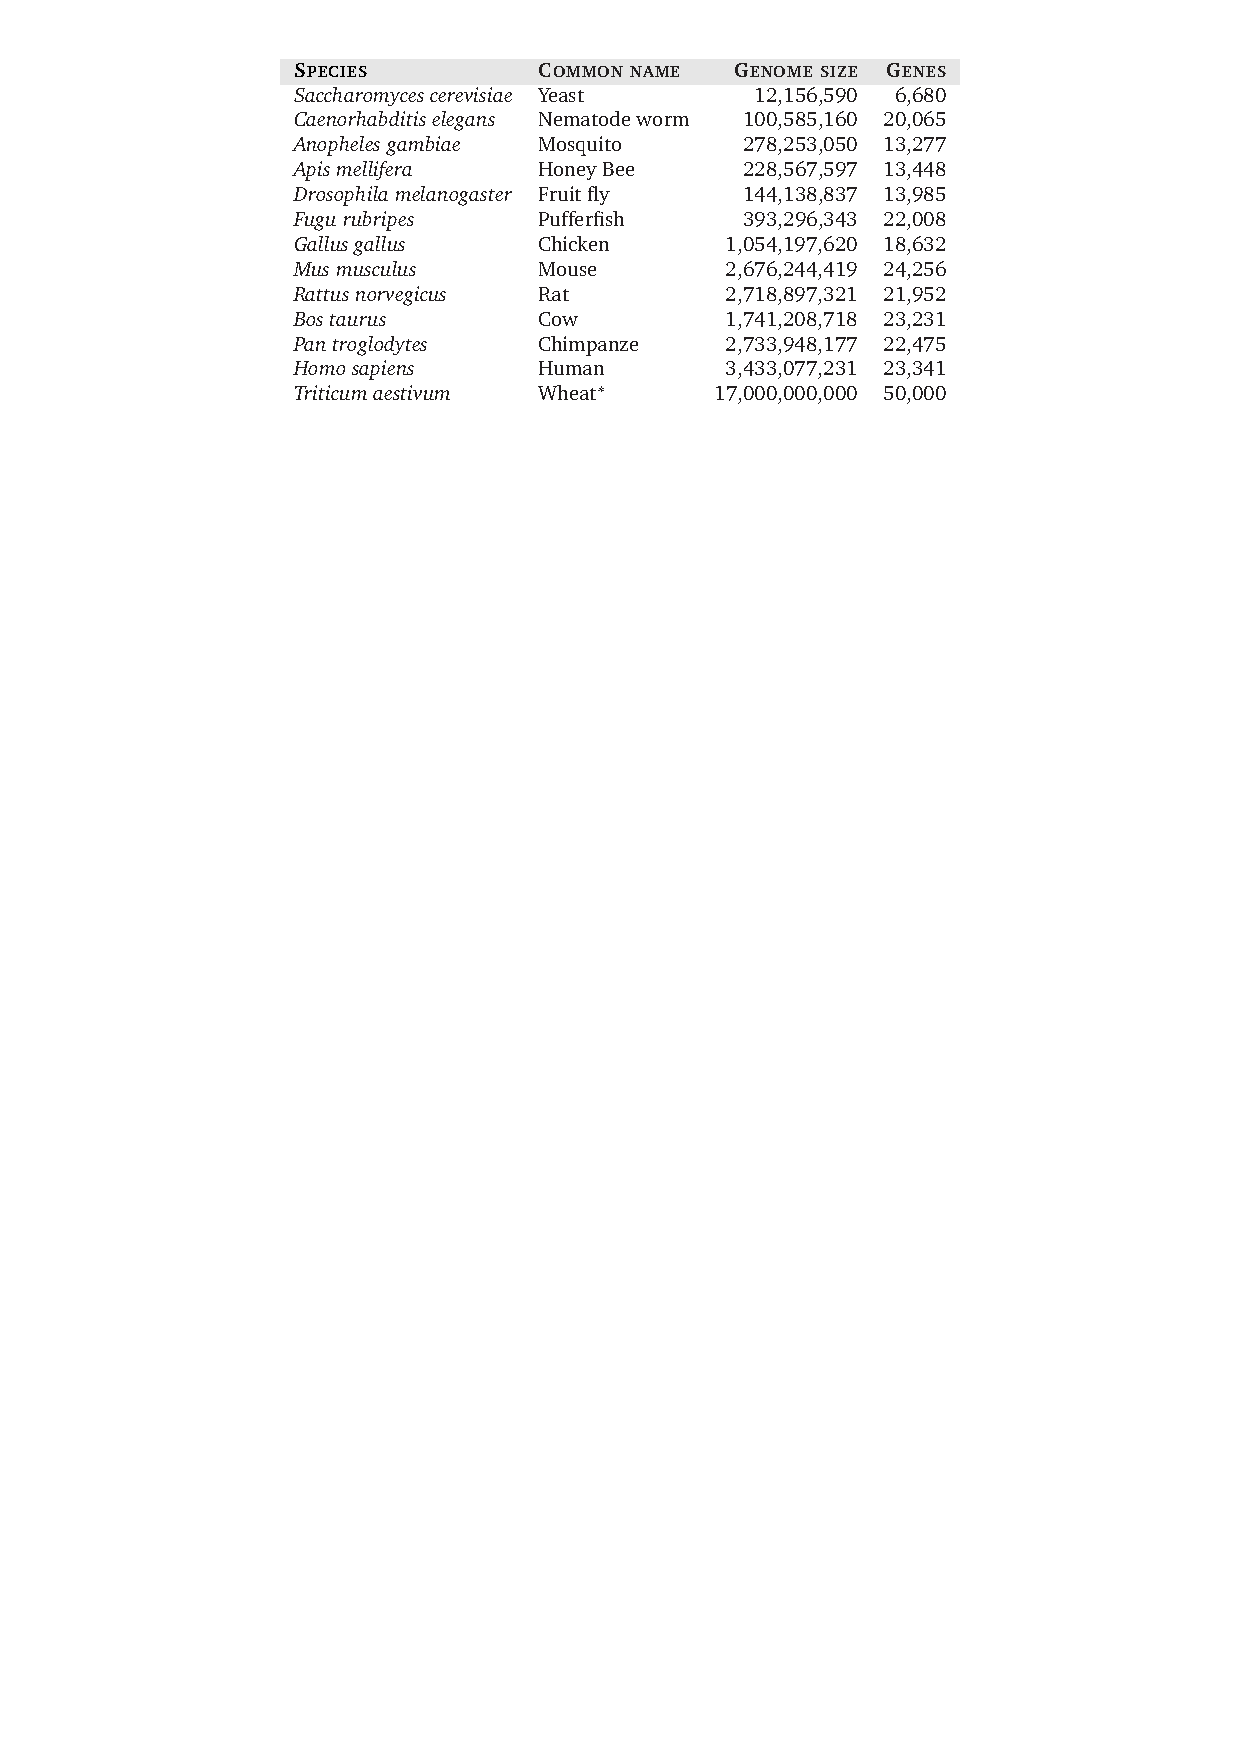
\includegraphics[bb=131 645 466 815,clip]{tables/gsizes}
\end{center}
\end{minipage}
\mycaption{tab:gsizes}% label
          {Comparison of the sizes of several eukaryotic genomes}% lof
          {Comparison of the sizes of several eukaryotic genomes.}% caption header
          {Data extracted from \ensembl{} (May, 2006). Estimated values for wheat.}
\end{center}
\end{table}

\noindent Broadly, bioinformatics tasks can be divided intro three categories:

\begin{menumerate}
\item
Implementation of databases to organize existing information from many areas of biological research
such as genomics, transcriptomics and proteomics, allowing the public scientific community to 
efficiently access the data and to avoid redundancy and multiplicity. Doubtlessly, the advent of 
internet has played a central role in the achievement of this challenge \citep{goodman:2002a}.
\item
Development of new algorithms and statistics that aid the analysis of the data such as sequence 
alignment methods, motif detection techniques, phylogenetic studies or protein folding simulation.
Advanced algorithmic methods and mathematical frameworks are essential to extract biological
knowledge from the databases.
\item
The analysis of such data and the interpretation of the results in a biologically meaningful 
manner to provide a more global perspective (new testable hypotheses) in future experimental designs. 
So far, it is far often easier to produce sequence data than to understand its function so that this 
is the most complicate of the three tasks \citep{bogusky:1998a,claverie:2000a,pearson:2001a}.
\end{menumerate}

\subsectionblue{Sequence databases}
\index{sequence!seqdb@databases} 

%%%%
% Figure 5: Genome composition 
%%%%
\begin{figure}[t!]
\begin{center}
\setlength{\fboxsep}{0pt}
\fbox{
\begin{tabular}{c}
\incgraph{width=0.6\linewidth}{ps/gcompo1}\\
\incgraph{width=0.6\linewidth}{ps/gcompo2}
\end{tabular}}
\mycaption{fig:gcompo}% label
          {The organization of the human genome}% lof
          {The organization of the human genome.}% caption header
          {(Top) A segment of the human genome.
           (Bottom) The contribution of different genomic elements to the human genome.
           Adapted from \citet{brown:1999a}.}
\end{center}
\end{figure}


A biological database is a large, organized body of persistent data designed to be queried
and retrieved in a very efficient manner by the scientific community. Because of the nature of the 
first data, ancient databases were merely collections of sequences of proteins distributed as a printed 
work \citep{dayhoff:1965a}. Nonetheless, the need for an electronic format became obvious just when the 
amount of sequences was unmanageable \citep{baxevanis:2005a,mount:2001a}. With substantial experimental 
sequencing improvements and the advent of DNA sequence databases initiated by the European Molecular 
Biology Laboratory (EMBL, Germany) and Los Alamos National Laboratory (LANL, United States), the 
number of available sequences experienced an exponential growth (see Figure \ref{fig:genbank}).

Major public nucleotide and protein sequence databases such as 
\embl{}
\index{EMBL} 
(\citealp{kulikova:2004a}, \webitemlink[embl]
    {\url{http://www.ebi.ac.uk/embl/}}
    {\db{European Molecular Biology Laboratory (EMBL)}}
    {%
      EMBL-nucleotide sequence database.
    }%
    {emblurl})
or \genbank{}\index{GenBank}\footnote{GenBank is now under the auspices of the National Center for Biotechnology Information (NCBI, United States).}
(\citealp{benson:2004a}, \webitemlink[genbank]
    {\url{http://www.ncbi.nlm.nih.gov/Genbank/index.html}}
    {\genbank{}}
    {%
       GenBank is the NIH genetic sequence database, an annotated 
       collection of all publicly available DNA sequences.
    }%
    {emblurl})
are repositories of sequences submitted by researchers in order to make them accessible for the
rest of the biological community. An accession number and a set of annotations are provided for
each sequence entry. Using flat files as a standard format, the features of each sequence are displayed 
in a simple format that divides each line of information into two elements: a field descriptor and a 
value. The popular \prog{FASTA} format 
\index{FASTA!fformat@format} 
is one of the \emph{de facto} standards that have been 
adopted to represent a sequence of nucleotides or amino acids (see Figure \ref{fig:gbentry} for an
example of a GenBank entry and the associated \prog{FASTA} file).

%%%%
% Figure 6: growth of genbank (web)
%%%%
\begin{figure}[t!]%
\begin{center}
\setlength{\fboxsep}{0pt}
%\fbox{
\incgraph{width=0.5\linewidth}{ps/gbgrowth}%}
\mycaption{fig:genbank}% label
          {Growth of the \genbank{} (1982-2004)}% lof
          {Growth of the \genbank{} (1982-2004).}% caption header
          {Adapted from \genbank{} (\webitemlink[genbank-stats]
    {\url{http://www.ncbi.nlm.nih.gov/Web/GenBank/genbankstats.html}}
    {\genbank{}}
    {Overview about the content of \genbank{}.}
    {genbankstatsurl}).}
\end{center}
\end{figure}

Because of the relative lack of control over the quality and quantity of the data stored in the 
sequence databases during the first years, there was soon a necessity to maintain collections of data
free of redundancy and errors constructed from the original repositories. Since then, numerous curated 
databases, also known as secondary databases, have appeared aiming to avoid any type of multiplicity and 
low quality data \citep{baxevanis:2005a}. 

%%%%
% Figure 7: Genbank entry
%%%%

\begin{figure}[t!]
\begin{center}
\setlength{\fboxsep}{0pt}

\begin{tabular}{cc}
\rotatebox{90}{\genbank{}} & 
\fbox{\begin{tabular}{c}
\incgraph{width=0.575\linewidth}{ps/gbentry1}\\
\incgraph{width=0.575\linewidth}{ps/gbentry2}
\end{tabular}}\\
& \\
\rotatebox{90}{\prog{FASTA}} & 
\fbox{\begin{tabular}{c}
\incgraph{width=0.575\linewidth}{ps/gbentry3}
	  \end{tabular}}
\end{tabular}
\mycaption{fig:gbentry}% label
          {An example of \genbank{} entry}% lof
          {An example of \genbank{} entry and a \prog{FASTA} sequence.}% caption header
          {}
\end{center}
\end{figure}

A successful example of these refined catalogues is the \refseq{} 
\index{RefSeq} 
collection (\citealp{pruitt:2005a},
\webitemlink[refseq]
    {\url{http://www.ncbi.nlm.nih.gov/RefSeq/}}
    {\db{The Reference Collection (RefSeq)}}
    {%
      The Reference Sequence (RefSeq) collection aims to provide a comprehensive, 
	  integrated, non-redundant set of sequences, including genomic DNA, transcript (RNA), 
	  and protein products, for major research organisms.
    }%
    {refsequrl}).
The major goal of this database is to provide a unique sequence for each molecule in the protein
synthesis pathway (DNA, mRNA and protein). To reduce the noise produced by the representation of 
a single biological entity with many entries in the sequence databases, each biological entity is 
represented only once in \refseq, maintaining a non-redundant repository.

\subsectionblue{Genomic databases}
\index{genome!gdb@databases}

Once the complete assembly of first eukaryotic genomes such \Scer{} \citep{goffeau:1996a} or 
\Dmel{} \citep{adams:2000a} was achieved, the principal focus of computational biology research 
shifted from individual sequences to chromosomes and whole genomes. With the release of the human 
genome \citep{lander:2001a,venter:2001a,ihgsc:2004a}, it became necessary to introduce an important 
change in the way the assemblies and the genome annotations were presented. \index{genome!genrelease@projects} 
Finally, the recent availability of the mouse genome \citep{waterston:2002a}, the chicken 
genome \citep{hillier:2004a} 
and the sequencing of other model organisms has augmented the need for a new kind of tools to permit 
the annotation and comparison of many genomes in a more sophisticate form. In addition, support for 
genomes that have not been finished yet has also been crucial (archives of traces and preview releases).

\noindent There are three well established genome browsers that aim to fulfill this need:

\begin{mitemize}
\item
The \ensembl{} project \index{Ensembl} 
(\citealp{birney:2004a}, \webitemlink[ensembl genome browser]%
    {\url{http://www.ensembl.org/}}%
    {\ensembl{}}%
    {%
%%
    Ensembl is a joint project between EMBL - EBI and the 
	Sanger Institute  to develop a software system which produces 
	and maintains automatic annotation on selected eukaryotic genomes.
%%
    }%
    {ensemblurl}), %
a collaboration between the European Bioinformatics Institute and the Sanger Institute.
The main browser currently provides a set of gene, transcript and protein predictions for each
genome. Data is presented on pages called Views, each View showing a different level of detail.

\item
The \ucscgb{} \index{UCSC genome browser} 
(\citealp{karolchik:2003a}, \webitemlink[ucsc genome browser]%
    {\url{http://genome.ucsc.edu/}}%
    {\ucscgb{}}%
    {%
%%
	  This site contains the reference sequence and working draft assemblies for a 
	  large collection of genomes. It also provides a portal to the ENCODE project.
%%
    }%
    {ucscgburl}), %
produced by the University of California, Santa Cruz Genome Bioinformatics Group. 
It serves annotations for many eukaryotic genomes, presenting the information in the 
form of tracks. Each track corresponds to a certain genomic feature. 

\item
The \ncbimv{} 
(\citealp{wheeler:2005a}, \webitemlink[ncbi map viewer]%
    {\url{http://www.ncbi.nlm.nih.gov/mapview/}}%
    {\ncbimv{}}%
    {%
%%
    The Entrez Map Viewer is a software component of Entrez Genomes. It allows you to 
	view an organism's complete genome, integrated maps (when available) for each chromosome, 
	and sequence data for a region of interest.
%%
    }%
    {ncbigburl}), %
provides maps for a lot of organisms, many of them without finished assembly. The browser 
is tightly linked to most services of the NCBI web. The information is displayed using  
maps. Maps are vertical representations of annotations along a given chromosome. There is a 
map associated to each genomic feature.

\end{mitemize}

The core of the three browsers is the internal gene annotation pipeline that must be executed on
every new sequence assembly of each genome. Genes are annotated according to experimental 
evidence and computational predictions. Comparisons between different genomes are also employed to 
improve the results. Moreover, other genome features such as regulatory regions, repeats, transcripts
or sequencing markers are integrated with the sequence and the annotated genes. In Figure 
\ref{fig:gbrowsers}, a screenshot of the same gene displayed in the \ucscgb{} and \ensembl{} is shown.

%%%%
% Figure 8: Genomic browsers
%%%%
% GBROWSERS: 
\begin{figure}[t!]
\begin{center}
\setlength{\fboxsep}{0pt}
\begin{tabular}{cc}
\rotatebox{90}{\centering\ucscgb{}} & \fbox{\incgraph{width=0.9\linewidth,height=8.75cm}{ps/gbrowsers1}}\\
 & \\
\rotatebox{90}{\centering \ensembl{}}& \fbox{\incgraph{width=0.9\linewidth,height=8.75cm}{ps/gbrowsers2}}
\end{tabular}
\mycaption{fig:gbrowsers}% label
          {The human URO-D gene in the \ucscgb{} and \ensembl{}}% lof
          {The human URO-D gene in the \ucscgb{} and \ensembl{}.}% caption header
          {}
\end{center}
\end{figure}


\subsectionblue{Data integration (integromics)}

The biological information that can be now accessed in the databases has not been generated
during a continuous process with several steps following an increasing order of complexity. On the 
contrary, different and discontinuous waves of genome-wide data have overlapped to form the current
body of knowledge. The new high-throughput technologies that have arisen in the last decades have
been the main catalyst conducing the progress. The first wave was the large-scale production of 
fragments of transcripts also named expressed sequence tags (ESTs). \index{ESTs}
The second wave was originated by
the sequencing of whole microbial organisms and was quickly followed by the achievement of the genomic
sequence of many eukaryotic organisms including human. Simultaneously, microarrays and
related technology have produce an overwhelming amount of expression data for which new analysis 
methods are still being designed \citep{searls:2000a}. 

In the near future, new waves of information are expected, such as the generation of maps of 
functional SNPs (see section \ref{sec:pgera}), or the complex interaction networks produced by 
emerging systems biology \citep{kitano:2002a}. Information technologies have adapted to the changing
nature of the new data. With every explosion of new knowledge, previous procedures have been reused 
and others have been created from scratch to integrate the new type of data with the already 
existing information. The power of data integration arises not from the value of every separate kind of 
information but from the gain produced by the fusion of all of them. With the advent of more
waves of knowledge, integromics will become absolutely essential to manage an amount of 'Omic' 
information that will exceed exabyte ($10^{18}$ bytes) quantities \citep{searls:2005a}.

Biological databases are essential resources used by biologists around the world. However, each one
contains only a subset of biological knowledge. This specificity increases the complexity of finding 
the answer for the majority of questions. Thus, several databases must be explored in order to obtain
the expected results. Cross-database queries require complex mechanisms of data integration that are
often not implemented properly \citep{stein:2003a}. 

For instance, the name of biological objects such as genes in the genomic browsers of several species 
(e.g. Rad24, rad24 or RAD24) or the definition of simple entities such as the gene concept 
(considering only transcript or transcript and regulatory region) can be a source of disagreement. 
Consequently, the role of ontologies to facilitate data integration must not be neglected. The 
popular \go{} \index{Gene Ontology (GO)}
(\citealp{tgoc:2000a}, \webitemlink[gene ontology]%
    {\url{http://www.geneontology.org}}%
    {\go{}}%
    {%
%%
	 The Gene Ontology (GO) project is a collaborative effort to address the need for consistent 
	 descriptions of gene products in different databases. The Gene Ontology project provides a 
	 controlled vocabulary to describe gene and gene product attributes in any organism.
%%
    }%
    {gourl}) 
establishes a taxonomy of controlled vocabulary that is used by most genome annotation projects
to uniformly annotate the function of genes.

\noindent There are several ways in which databases developers have tried to integrate databases:
\begin{mitemize}
\item
Link integration. Hypertext links are used to jump from one database to another. Although it is
the most popular solution, it has two severe drawbacks: links are vulnerable to name ambiguities and 
their updating is laborious.
\item
View integration. An environment around the databases is built to create the illusion of a unique
resource formed by different sources of data with specific data drivers to retrieve the information. 
The complexity of such a design is the main disadvantage of this strategy.
\item
Data warehousing. Merge all of the databases into a single database. Due to the continuous updating
of biological databases and the impossibility of reusing the software from one release to the next,
this approach is unfeasible in practice.
\end{mitemize}

%%%%%%%%%%%%%%%%%%
\sectionblue{The post-genomic era}\label{sec:pgera}

\subsectionblue{New forms of investigation}

The availability of many genomes and the improvement of very large-scale gene expression experiments
have substantially modified the form in which current research is focused \citep{searls:2005a}. 
The classical hypothesis-driven research paradigm, in which a specific proposition is addressed over 
a set of targets, is progressively being substituted with data-driven investigations, in which high-throughput 
explorations are performed typically over the whole collection of genes of an organism to detect
previously unknown relationships. Data-diving excursions have several risks derived from their 
massive exploration. Correct normalization and replication of the results is extremely difficult.
In addition, there is usually a high probability of finding pure artefactual relations due to the 
low signal/noise ratio observed in such experiments \citep{searls:2005a}.

Much effort must be invested to make bioinformatics become part of the wet-dry cycles of research
\citep{searls:2000a}. Such discovery processes occur whenever a computational method is linked to a 
biological one, such that predictions from the former can be tested at the bench, within a feedback 
strategy. Once the computational candidates have been delivered, they should be monitored during the 
experimental pipeline, using such results to refine the original computational model \citep{searls:2000a}.

\subsectionblue{Genomics and health}

Virtually every human illness has a hereditary component \citep{collins:2001a}. The characterization 
of the genetic determinants of disease would provide remarkable opportunities for clinical medicine. 
Current clinical practice is still based on phenotypic criteria to define most diseases rather than
studying the underlying mechanisms. Obtaining the sequence of the human genome is only the end of the 
beginning \citep{collins:2001a}. Among the grand challenges to achieve after the sequence of many
genomes is available is the development of strategies for identifying the genetic contributions to 
disease and the gene variants that promote good health and resistance to disease \citep{collins:2003a}. 
Progress is slow but evidence suggests that while public health and antibiotics have played the major 
roles in the past 50 years, the next 50 are likely to belong to genetics and molecular medicine 
\citep{bell:2003a}.

Simple changes in our genes can lead to disease. 
\index{gene!geneillness@genes and illness}
Single gene mutations, which are already commonly 
used in diagnostic practice (genetic and disease markers), cause approximately $6,000$ inherited 
diseases also known as monogenic diseases. Disorders like cystic fibrosis, anemia or hemophilia 
affect millions of people worldwide. For more common diseases such as heart disease, diabetes, or 
Alzheimer's disease, the interplay of multiple genes and multiple non-genetic factors (environment 
effects) that contribute to disease susceptibility is still being characterized (GSK report: Genes 
and diseases, \webitemlink[gsk]%
    {\url{http://genetics.gsk.com/link.htm}}%
    {Genetics GSK report: Genes and diseases}%
    {%
%%
    GlaxoSmithKline educational resource.
%%
    }%
    {gskurl},
NHGRI/NIH report: Genetics, the Future of Medicine, \webitemlink[nhgri]%
    {\url{www.nhgri.nih.gov}}%
    {NHGRI/NIH report: Genetics, the Future of Medicine}%
    {%
%%
    National Human Genome Research Institute.
%%
    }%
    {nhgriurl}).

For example, loss of control in the growth mechanisms of cells results in cancer. 
\index{cancer} \index{gene!gcancer@cancer}
The transformation of a normal cell into a cancerous one is caused by molecular changes that underly
growth-signal independence, insensitivity to anti-growth signals, evasion of immunosurveillance,
apoptosis evasion, unlimited replicative potential, tissue invasion and metastasis. 
These molecular changes involving several genes can be produced by certain
events that alter the genome such as point mutations, gene amplifications and deletions, and 
chromosomal translocations. The intimate relationship between cancer and genome sequencing projects
has originated the recent launch of several cancer genome projects \citep{strausberg:2003a}.

%%%%
% Figure 9: Classes of SNPs
%%%%%
\begin{figure}[t!]%
\begin{center}
\setlength{\fboxsep}{0pt}%
%\fbox{
\begin{tabular}{cc}
\incgraph{width=0.25\linewidth,height=6cm}{ps/snp1} &
\incgraph{width=0.25\linewidth,height=6cm}{ps/snp2}\\
\end{tabular}%}
\mycaption{fig:snps}% label
          {Using SNPs to locate susceptibility genes}% lof
          {Using SNPs to locate susceptibility genes.}% caption header
          { (Left) SNP profiling of two groups of people.
            (Right) Categories of SNPs according to their location.
            Adapted from GSK report: Genes and diseases.}
\end{center}
\end{figure}%

\subsectionblue{Pharmacogenomics}
\index{pharmacogenomics}

Before the end of this century, shortly after a person is born, her genotype will be saved at her 
physician's office to record the presence  or absence of specific variations known to be relevant 
for assessing disease susceptibility and prediction response to drug types. Biomolecular profiling 
throughout her life will complement this information to provide recommendations about life-style 
or diet and to detect early stages of a disease. This future scenario in which personalized medicine
and therapy are present in our lives to increase the quality of life and life-span is not 
unrealistic \citep{sander:2000a}. 

In 1998, adverse drug reactions produced over $100,000$ deaths in the United States, being one of the
leading causes of hospitalization and death. The one-size-fits-all formula typically works for only 
$60$\% of the population at best. The way a person responds a drug (positively or negatively) 
is a complex trait influenced by many different genes. Pharmacogenomics \footnote{The related term 
pharmacogenetics appeared in the 1950s describing the study of inherited genetic variation in drug 
metabolism and response.} is the science that examines the gene variations that dictate drug response
and explores how to use them to predict whether a patient will have a good reaction, a bad reaction
or no reaction to a given drug 
(\citealp{evans:1999a}, NCBI report: pharmacogenomics,
\webitemlink[ncbi a science primer pharmacogenomics]
    {\url{http://www.ncbi.nlm.nih.gov/About/primer/pharm.html}}
    {\db{NCBI} A Science Primer (pharmacogenomics)}
    {%
      A Basic Introduction to the Science Underlying NCBI Resources.
    }%
    {ncbiinfothreeurl}).

First studies focused on the broadest categories of inheritance: ethnicity, geography, language and
race. Several SNPs mapping projects are working to provide a catalogue of observed 
one-letter differences between individuals in a population. SNPs are present throughout
\index{SNP!SNPdis@distribution} 
the human genome with an average frequency of $1$ per $1,000$ base pairs. Their relatively even 
distribution make them valuable as genetic markers. To be helpful, the polymorphism must be shared 
by at least $1$\% of the population tested, thus becoming a shared SNP. Mutations are less
common differences, occurring in a smaller proportion.

With these SNP maps, genetic profile comparison of patients who may suffer from serious side effects 
and those that may not, might be useful to detect one or more SNPs that differ between both groups. Careful 
examination of the small area of the genome where the differences are found will classify them
into functional and non-functional SNPs (see Figure \ref{fig:snps}). 
\index{SNP!SNPclas@classes} 
For instance, SNPs found in 
protein coding regions (cSNPs) would be good candidates to elaborate a hypothetic explanation of
the observed drug response as long as they produce a change in the translated amino acid sequence 
(non synonymous changes).

The haplotype is the set of closely related genes (alleles) that tend to be inherited together as 
a single unit. \index{haplotype} 
The International HapMap Project is currently in charge of developing the haplotype 
map of the human genome \citep{tihc:2003a}. The official repository of SNPs mined by this project
is the NCBI \dbsnp{} database
(\webitemlink[dbSNP]%
    {\url{http://www.ncbi.nlm.nih.gov/SNP/}}%
    {\dbsnp{}}%
    {%
%%
     The NCBI database of SNPs.
%%
    }%
    {dbsnpurl}) %% 
that contains information for other genomes as well. SNP annotation is also integrated in the 
genomic browsers explained in Section \ref{sec:gera}. For further information about sequence
polymorphisms, see \citet{mullikin:2005a}.

%%%%%%%%%%%%%%%%%%
%%% References for this chapter
%%% ENCERRAR ENTRE LLAVES PARA EVITAR PROBLEMAS
\bibliographystyle{plainnat}
{\bibliography{sections/bibliography}}
